\chapter*{Zeitplan}


\begin{sidewaysfigure}[!ht]
    \centering
    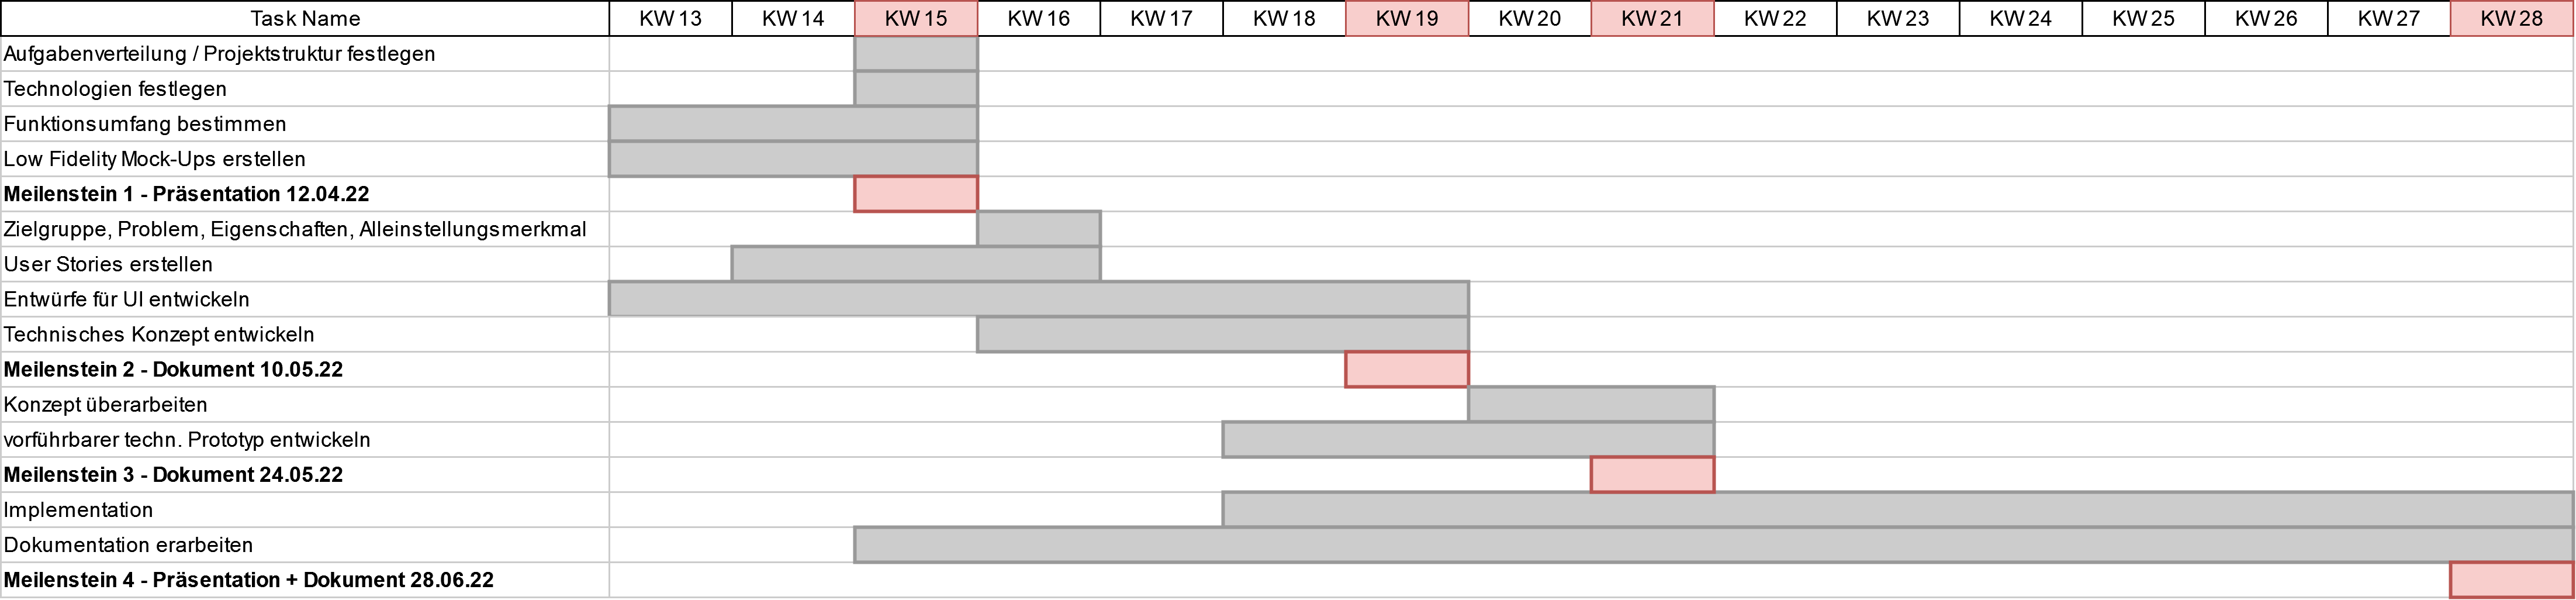
\includegraphics[width=0.6\textwidth]{Zeitplan_DeskPlanner.png}
    \caption{Zeitplan}
    \label{fig:Zeitplan}
\end{sidewaysfigure}

Der Zeitplan hangelt sich an den vorgegebenen Meilensteinen 1-4 entlang.\\
\textbf{Meilenstein 1 (12.04.22)}\\
Präsentation:
\begin{itemize}
    \item Aufgabenverteilung
    \item Projektmanagement
    \item Technologien
    \item Funktionsumfang
    \item UI-Entwürfe, z.B. Low Fidelity Mock-Ups
\end{itemize}

\vspace{0.03\textwidth}
\textbf{Meilenstein 2 (10.05.22)} \\
Dokumentation:
\begin{enumerate}
    \item Zielgruppe, Problem, Eigenschaften, Alleinstellungsmerkmal
    \item User Stories
    \item User Interface Entwürfe
    \item Technisches Konzept
    \begin{itemize}
        \item Verwendete Frameworks
        \item Softwarearchitektur
        \begin{itemize}
            \item UML-Verteilungsdiagramm des Gesamtsystems
            \item UML-Komponentendiagramm (jeweils für Client und Server)
        \end{itemize}
        \item Datenbank
        \begin{itemize}
            \item Entity Relationship Model
        \end{itemize}
    \end{itemize}
    \item UI-Entwürfe, z.B. Low Fidelity Mock-Ups
\end{enumerate}

\textbf{Meilenstein 3 (24.05.22)}

\textbf{Meilenstein 4 (28.06.22)}